\documentclass[12pt,
border=1pt]{standalone}
\usepackage{pgfplots}
\usepackage{amsmath}
\usepackage{amssymb}

\pgfplotsset{compat=newest,
	width=6cm, height=5cm,
	xtick pos=left, ytick pos=left,
	%            scaled x ticks=real:1e-6,
}
% Kernel 2 FP64
\begin{document}
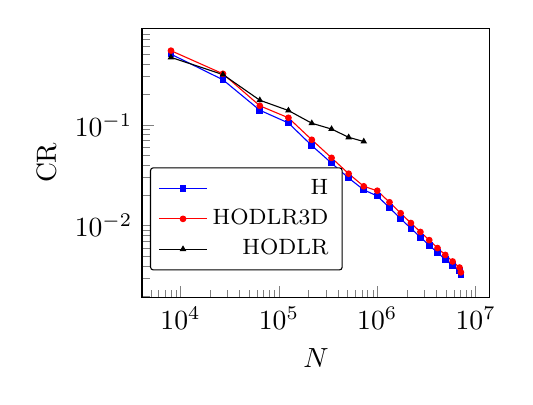
\begin{tikzpicture}[every mark/.append style={mark size=1pt}]
	\begin{axis}[xlabel={$N$},
	ylabel={CR},
%		legend pos=south east,
		legend style={
                at={(0.3,0.1)},
               anchor=south,
               legend columns=1,
               cells={anchor=east},
               font=\footnotesize,
               rounded corners=1pt,
               },
		xmode = log,
	    ymode = log,
	   % xmin = 1e3,
	   % xmax = 1e6,
	   % ymin = 1e-10,
	   % ymax = 1e-0,
	   % xtick={1e-10, 1e-8, 1e-6,  1e-4,  1e-2},
	   % ytick={1e-8, 1e-6,  1e-4,  1e-2, 1e-0}
		]

		%Vaishnavi
		\addplot[
		color=blue,
		mark=square*,
		] coordinates {
(8000,0.502707)
(27000,0.280057)
(64000,0.139726)
(125000,0.104397)
(216000,0.062265)
(343000,0.041743)
(512000,0.029662)
(729000,0.022654)
(1000000,0.019699)
(1331000,0.015056)
(1728000,0.011699)
(2197000,0.009397)
(2744000,0.007687)
(3375000,0.006385)
(4096000,0.005408)
(4913000,0.004623)
(5832000,0.004021)
(6859000,0.003538)
(7077888,0.003243)
		};
		%Zhao
		\addplot[
		color=red,
		mark=*,
		] coordinates {
(8000,0.544637)
(27000,0.321098)
(64000,0.154500)
(125000,0.117509)
(216000,0.071118)
(343000,0.047071)
(512000,0.032757)
(729000,0.024578)
(1000000,0.022203)
(1331000,0.017068)
(1728000,0.013292)
(2197000,0.010621)
(2744000,0.008660)
(3375000,0.007187)
(4096000,0.005995)
(4913000,0.005126)
(5832000,0.004415)
(6859000,0.003841)
(7077888,0.003444)
		};
		
		\addplot[
		color=black,
		mark=triangle*,
		] coordinates {
(8000,0.467232)
(27000,0.315538)
(64000,0.175540)
(125000,0.138782)
(216000,0.103787)
(343000,0.090862)
(512000,0.075243)
(729000,0.068362)
		};
		\legend{H, HODLR3D, HODLR}
	\end{axis}
\end{tikzpicture}
\end{document}